\documentclass[border=2pt]{standalone}
\usepackage[dvipsnames]{xcolor}
\usepackage{tikz}
\usetikzlibrary{positioning,decorations.pathreplacing,fit}
\usetikzlibrary{decorations.markings,arrows.meta,shapes.arrows}
\usetikzlibrary{calc}

\definecolor{darkgreen}{RGB}{0,128,80}

\graphicspath{{./images/}}

\begin{document}


\begin{tikzpicture}[
	arrow double line/.style={
		double distance = 17pt,
	    postaction = {
    		draw = white,
	 	    line width = 17pt,
	 	    shorten <= -.1pt,
	 	    shorten >= -.1pt,	
	    },
	    postaction={
	    	decorate, 
	    	decoration = {
	    		markings, 
	    		mark=at position 0 with {
	    			\arrow[xshift=24.6pt]{Straight Barb[reversed,length=-1pt 0.7]}
	    		}
	    	}
	    },
	    postaction={
   	    	decorate, 
   	    	decoration = {
   	    		markings, 
   	    		mark=at position 1 with {
   	    			\arrow[xshift=10.6pt]{Straight Barb[length=-1pt 0.7]}
   	    		}
   	    	}
 	    },
   		shorten <= 12.2, 	
   		shorten >= 11.4,
   		thick,
	},
	mybrace/.style= {
		decorate, decoration={brace,amplitude=5pt,raise=5pt}, line width=0.7pt
	},
	mybrace mirror/.style= {
			decorate, decoration={brace,amplitude=5pt,raise=5pt,mirror}, line width=0.7pt
	},
	every node/.style={
		font=\bfseries
	}
	]

	

		
	\node[] (client) {\underline{Client}};
	\node[right = 5.0 of client] (AP) {\underline{Authenticator}};
	\node[right = 4.2 of  AP] (AS) {\underline{Server}};
	\def\InterMsgSpaceVertical{1}

	\node[inner sep=0pt, xshift=0cm,yshift=1.3cm] (laptop_icon) at (client) {\reflectbox{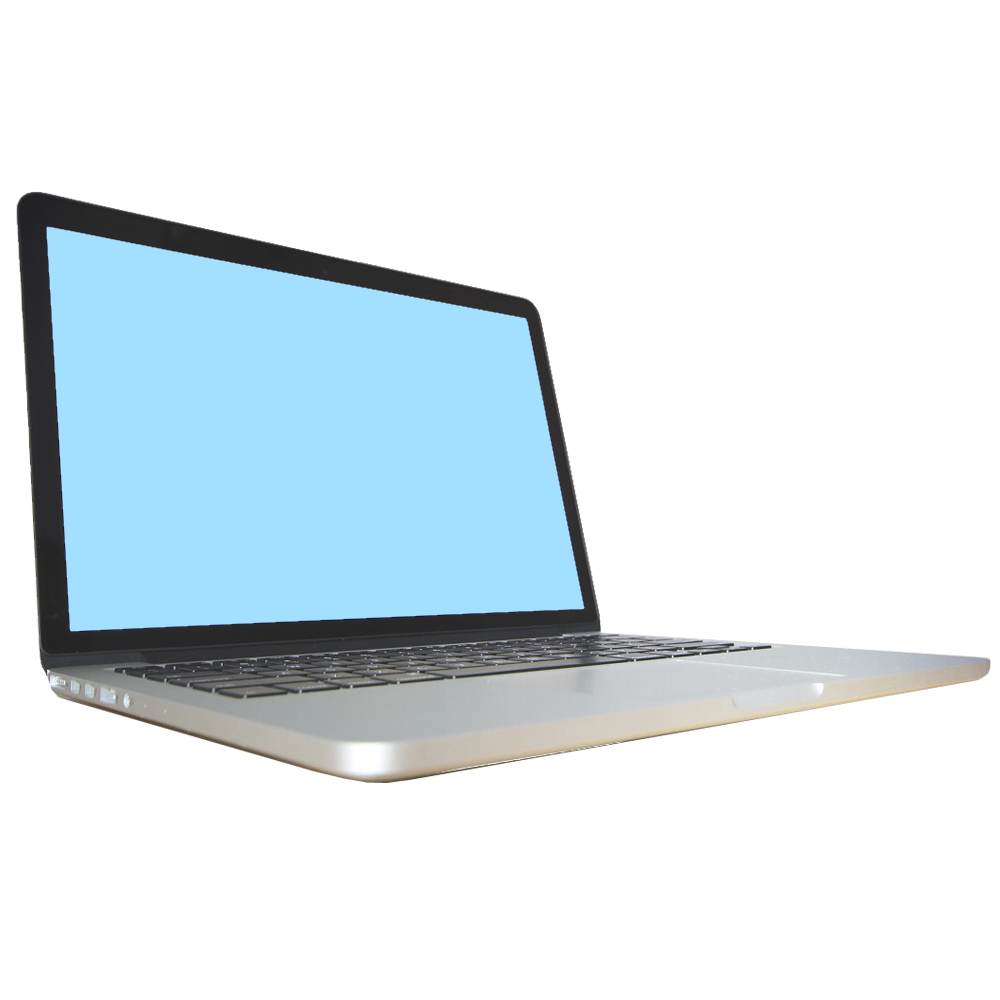
\includegraphics[width=.19\textwidth]{laptop4}}};
	\node[inner sep=0pt, xshift=-0.0cm,yshift=1.55cm] (AP_icon) at (AP) {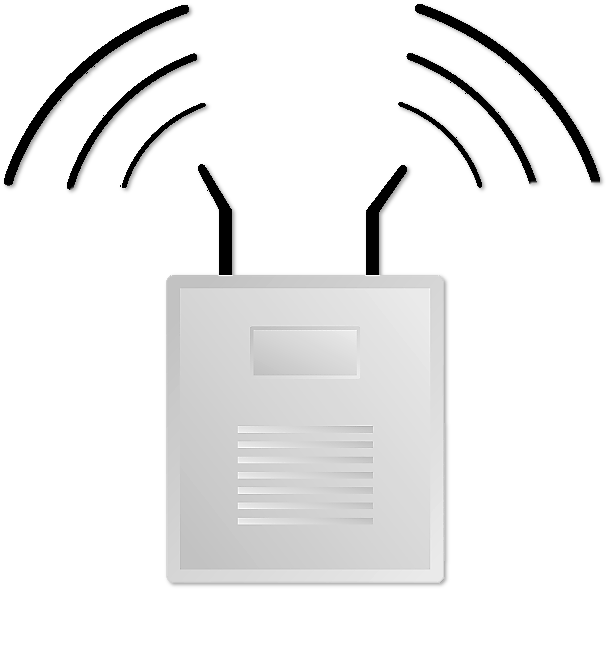
\includegraphics[width=.18\textwidth]{AP}};
	\node[inner sep=0pt, xshift=0.05cm,yshift=1.5cm] (server_icon) at (AS) {
\includegraphics[width=.11\textwidth]{server}};
		
	\foreach \i in {1,...,8} {
		\coordinate[below = \InterMsgSpaceVertical * \i of client] (c\i) {};
		\coordinate[below = \InterMsgSpaceVertical * \i of AP] (ap\i) {};
		\coordinate[below = \InterMsgSpaceVertical * \i of AS] (as\i) {};
	}	
	


	\draw[arrow double line,red] (c1) -- node (EAP) {EAP method (EAP-TLS)} (as1);

	\draw[arrow double line,blue] (ap2) -- node[] (AAA) {Key-transport (RADIUS)} (as2);

	\draw[arrow double line,darkgreen] (c3) -- node {Link-layer protocol (IEEE 802.11)} (ap3);
	
	\path (client) -- node[yshift = -18pt] {$\longleftarrow$ Link layer $\longrightarrow$} (AP);
	
	\path (AP) -- node[yshift = -18pt] {$\longleftarrow$ IP layer $\longrightarrow$} (AS);
 
	

\end{tikzpicture}


\end{document}